\documentclass[]{beamer}
\usetheme[framenumber,totalframenumber]{UniversiteitGent}



\usepackage{manfnt}
\usepackage{minted}
\usepackage{pgfplots}
\usepackage{xspace}

% TikZ addons
\usepackage{tikz-cd}
\usepackage{tikz-qtree}
\usepackage{tqft}

\pgfplotsset{width = 7cm, compat = 1.8}
\usetikzlibrary{backgrounds, calc, decorations.markings, intersections, snakes, through, trees}

\newcommand\TikZ{Ti\textit{k}Z\xspace}

\def\Point{36.9}

\includeonly{tikz-extensions}

\begin{document}

\begin{frame}
  \frametitle{Waarom figuren maken in \LaTeX?}

  \begin{itemize}
    \item[+] aanpasbaarheid
      \begin{enumerate}
        \item je document opnieuw builden maakt de afbeelding opnieuw: wijzigingen aanbrengen is dus even gemakkelijk als \LaTeX-code wijzigen
        \item je hebt geen externe software nodig (!)
      \end{enumerate}
    \item[+] consistentie
      \begin{enumerate}
        \item lettertypes, kleuren, tekstgroottes, \ldots zijn overal hetzelfde
      \end{enumerate}
  \end{itemize}
\end{frame}

\begin{frame}
  \frametitle{Waarom figuren maken in \TikZ?}
  \begin{exampleblock}{}
    \mintinline{latex}|Making Greek letters is as easy as $\pi$.|

    Making Greek letters is as easy as $\pi$. 
    \vskip5mm
    \hspace*\fill{---Leslie Lamport, \LaTeX: A Document Preparation System}
  \end{exampleblock}
  \pause
  \begin{exampleblock}{}
    \mintinline{latex}|Drawing an orange circle is as easy as|
    \mintinline{latex}|\tikz \fill[orange] (1ex,1ex) circle (1ex);.|

    Drawing an orange circle is as easy as \tikz \fill[orange] (1ex,1ex) circle (1ex);.
    \vskip5mm
    \hspace*\fill{---Pieter Belmans}
  \end{exampleblock}
\end{frame}

\begin{frame}
  \frametitle{Wat is \TikZ?}

  \TikZ is een recursief acroniem voor
  \begin{center}
    \TikZ ist \emph{kein} Zeichenprogramm
  \end{center}
  \pause
  Dit betekent vooral dat \TikZ niet bedoeld is om in te tekenen zoals in Paint, maar om ``vector graphics'' te produceren. Het is een tekentaal, geprogrammeerd in \LaTeX.
  \pause
  Eigenlijk is \TikZ een frontend voor PGF, Portable Graphics Format, soms wordt de combinatie PGF/\TikZ genoemd.
  \pause
  \begin{block}{Versies}
    Enkele maanden geleden is versie 3 uitgekomen, maar deze workshop is nog geschreven in 2.10 (de versie die ge\"installeerd is).
  \end{block}
\end{frame}

\begin{frame}
  \frametitle{Wat gaan we vandaag vooral \emph{niet} doen?}

  Dit is \emph{geen} grondige \TikZ-cursus:
  \begin{enumerate}
    \item ik ben verre van een expert
    \item de tijd is beperkt
    \item \TikZ is \emph{gigantisch}
    \item\pause ik ben verre van een expert
  \end{enumerate}
\end{frame}

\begin{frame}
  \frametitle{Wat gaan we vandaag dan \emph{wel} doen?}

  \begin{enumerate}
    \item korte introductie tot de syntax
    \item waar kunnen we informatie vinden?
    \item wat is er allemaal mogelijk?
  \end{enumerate}
  Ik wil dus vooral laten zien \emph{wat} er mogelijk is, niet \emph{hoe} je het moet doen. Daarvoor dienen handleidingen en de vele beschikbare voorbeelden.
\end{frame}



\section{Voorbeelden}

\begin{frame}
  \frametitle{\url{http://TeXample.net}}

  \begin{columns}
    \begin{column}{.4\textwidth}
      \begin{enumerate}
        \item 350+ voorbeelden
        \item gesorteerd in categorie\"en
        \item bestaat al 8 jaar
        \item heeft ook een lijst van interessante \LaTeX\ blogs
      \end{enumerate}
    \end{column}

    \begin{column}{.6\textwidth}
      \begin{flushright}
        \resizebox{7cm}{!}{%

\begin{tikzpicture}
  \path[mindmap,concept color=black,text=white]
    node[concept] {Computer Science}
    [clockwise from=0]
    child[concept color=green!50!black] {
      node[concept] {practical}
      [clockwise from=90]
      child { node[concept] {algorithms} }
      child { node[concept] {data structures} }
      child { node[concept] {pro\-gramming languages} }
      child { node[concept] {software engineer\-ing} }
    }  
    child[concept color=blue] {
      node[concept] {applied}
      [clockwise from=-30]
      child { node[concept] {databases} }
      child { node[concept] {WWW} }
    }
    child[concept color=red] { node[concept] {technical} }
    child[concept color=orange] { node[concept] {theoretical} };
\end{tikzpicture}

}

      \end{flushright}
    \end{column}
  \end{columns}
\end{frame}

\begin{frame}
  \frametitle{\url{http://PGFPlots.net}}

  \begin{columns}
    \begin{column}{.4\textwidth}
      \begin{enumerate}
        \item 50+ voorbeelden
        \item gesorteerd in categorie\"en
        \item bestaat nu een maand
      \end{enumerate}
    \end{column}

    \begin{column}{.6\textwidth}
      \begin{flushright}
        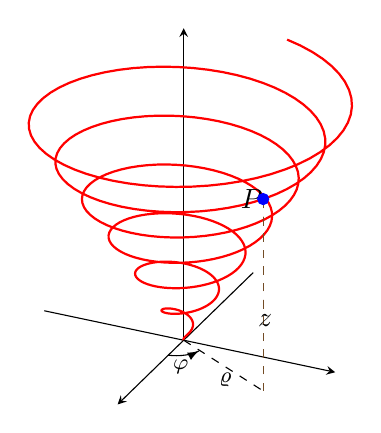
\begin{tikzpicture}
  \begin{axis}[
    view       = {-25}{-25},
    axis lines = middle,
    zmax       = 60,
    height     = 8cm,
    xtick      = \empty,
    ytick      = \empty,
    ztick      = \empty
  ]
  \addplot3+ [
    ytick      = \empty,
    yticklabel = \empty,
    domain     = 0:14.7*pi,
    samples    = 400,
    samples y  = 0,
    mark       = none,
    thick,
    red,
  ]
  ( {x*sin(0.28*pi*deg(x))},{x*cos(0.28*pi*deg(x)},{x});
  \addplot3+ [
    mark options = {color=blue},
    mark         = *
  ] 
  coordinates {({\Point*sin(0.28*pi*deg(\Point))},
    {\Point*cos(0.28*pi*deg(\Point)}, {\Point})};
  \addplot3+ [
    domain    = 0:12*pi,
    samples   = 100,
    samples y = 0,
    mark      = none,
    dashed,
  ]  
  ( {\Point*sin(0.28*pi*deg(\Point))}, {\Point*cos(0.28*pi*deg(\Point)}, {x} );
  \addplot3[
    mark=none,
    dashed
  ]
  coordinates {(0,0,0) ({\Point*sin(0.28*pi*deg(\Point))},
    {\Point*cos(0.28*pi*deg(\Point)}, {0})};
  \draw[
    radius = 80,
    decoration = {
      markings,
      mark= at position 0.99 with {\arrow{latex}}
    },
    postaction=decorate
  ] 
  (axis cs:0,10,0) arc[start angle=80,end angle=14] (axis cs:14,0,0);
  \node at (axis cs:20,0,30) {$P$};
  \node at (axis cs:24,0,7) {$z$};
  \node [font=\footnotesize] at (axis cs:20,17,0) {$\varrho$};
  \node [font=\footnotesize] at (axis cs:6,15,0) {$\varphi$};
  \end{axis}
\end{tikzpicture}

      \end{flushright}
    \end{column}
  \end{columns}
\end{frame}



\section{PGF/TikZ aan de hand van een voorbeeld}

\begin{frame}
  \frametitle{Uitgewerkt voorbeeld: een gelijkzijdige driehoek}

  In de \emph{Elementen van Euclides} (3e eeuw voor Christus) worden vele constructies in vlakke meetkunde beschreven. We gaan nu een voorbeeld uit de Ti\textit{k}Z manual bespreken:
  \begin{quote}
    Hoe construeren we een gelijkzijdige driehoek op een gegeven lijnstuk?
  \end{quote}

  \pause
  \centering
  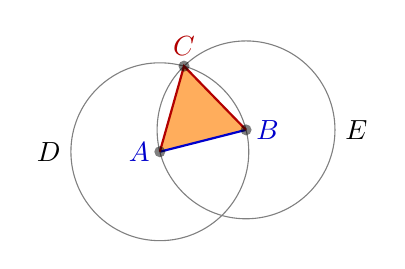
\begin{tikzpicture}[thick,help lines/.style={thin,draw=black!50}]
  \def\A{\textcolor{input}{$A$}}
  \def\B{\textcolor{input}{$B$}}
  \def\C{\textcolor{output}{$C$}}
  \def\D{$D$}
  \def\E{$E$}

  \colorlet{input}{blue!80!black}
  \colorlet{triangle}{orange!80!white}
  \colorlet{output}{red!70!black}

  \coordinate [label=left:\A]  (A) at ($ (0,0) + .1*(rand,rand) $);
  \coordinate [label=right:\B] (B) at ($ (1.25,0.25) + .1*(rand,rand) $);

  \draw [input] (A) -- (B);

  \node [name path=D,help lines,draw,label=left:\D]
    (D) at (A) [circle through=(B)] {};
  \node [name path=E,help lines,draw,label=right:\E]
    (E) at (B) [circle through=(A)] {};

  \path [name intersections={of=D and E,by={[label=above:\C]C}}];

  \draw [output] (A) -- (C) -- (B);

  \foreach \point in {A,B,C}
    \fill [black,opacity=.5] (\point) circle (2pt);

  \begin{pgfonlayer}{background}
    \fill[triangle!80] (A) -- (C) -- (B) -- cycle;
  \end{pgfonlayer}
\end{tikzpicture}

\end{frame}

\begin{frame}
  \frametitle{Stappenplan}

  \begin{columns}
    \begin{column}{.5\textwidth}
      \begin{enumerate}
        \item het lijnstuk $AB$
        \item de cirkels rond $A$ en $B$
        \item het snijpunt
        \item de driehoek
      \end{enumerate}
    \end{column}
    \begin{column}{.5\textwidth}
      \centering
      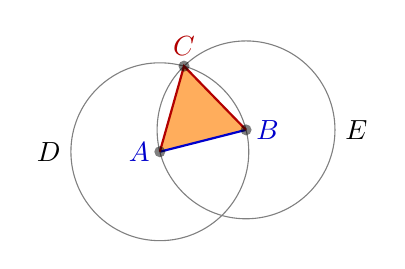
\begin{tikzpicture}[thick,help lines/.style={thin,draw=black!50}]
  \def\A{\textcolor{input}{$A$}}
  \def\B{\textcolor{input}{$B$}}
  \def\C{\textcolor{output}{$C$}}
  \def\D{$D$}
  \def\E{$E$}

  \colorlet{input}{blue!80!black}
  \colorlet{triangle}{orange!80!white}
  \colorlet{output}{red!70!black}

  \coordinate [label=left:\A]  (A) at ($ (0,0) + .1*(rand,rand) $);
  \coordinate [label=right:\B] (B) at ($ (1.25,0.25) + .1*(rand,rand) $);

  \draw [input] (A) -- (B);

  \node [name path=D,help lines,draw,label=left:\D]
    (D) at (A) [circle through=(B)] {};
  \node [name path=E,help lines,draw,label=right:\E]
    (E) at (B) [circle through=(A)] {};

  \path [name intersections={of=D and E,by={[label=above:\C]C}}];

  \draw [output] (A) -- (C) -- (B);

  \foreach \point in {A,B,C}
    \fill [black,opacity=.5] (\point) circle (2pt);

  \begin{pgfonlayer}{background}
    \fill[triangle!80] (A) -- (C) -- (B) -- cycle;
  \end{pgfonlayer}
\end{tikzpicture}

    \end{column}
  \end{columns}
\end{frame}

\begin{frame}
  \frametitle{Euclides: de configuratie}
  
  \inputminted[fontsize = \scriptsize]{latex}{tikz/triangle/configuration.tikz}

  \TikZ bevat vele libraries die bepaalde zaken gemakkelijker maken. In dit voorbeeld zullen we er vier gebruiken.
\end{frame}

\begin{frame}[fragile]
  \frametitle{Euclides: het lijnstuk $AB$ (1)}

  \begin{columns}
    \begin{column}{.67\textwidth}
      \inputminted[fontsize = \scriptsize]{latex}{tikz/triangle/1a.tikz}
    \end{column}
    \begin{column}{.33\textwidth}
      \begin{tikzpicture}
  \coordinate (A) at (0,0);
  \coordinate (B) at (1.25,0.25);
  \draw[blue] (A) -- (B);
\end{tikzpicture}

    \end{column}
  \end{columns}

  \footnotesize
  \begin{enumerate}
    \item\pause \mintinline{latex}|\draw| is het commando om iets te tekenen
    \item\pause \mintinline{latex}|--| is een gewone lijn tussen twee punten
    \item\pause we konden ook \mintinline{latex}|\draw[blue] (0,0) -- (1.25,0.25);| gebruiken, maar nu kunnen we de co\"ordinaten herbruiken
  \end{enumerate}
  \pause
  \begin{block}{Volgende stap}
    Hoe voegen we namen van punten toe?
  \end{block}
\end{frame}

\begin{frame}
  \frametitle{Euclides: het lijnstuk $AB$ (2)}

  \begin{columns}
    \begin{column}{.67\textwidth}
      \inputminted[fontsize = \scriptsize]{latex}{tikz/triangle/1b.tikz}
    \end{column}
    \begin{column}{.33\textwidth}
      \begin{tikzpicture}
  \coordinate[label=left:\textcolor{blue}{$A$}]
    (A) at (0,0);
  \coordinate[label=right:\textcolor{blue}{$B$}]
    (B) at (1.25,0.25);

  \draw[blue] (A) -- (B);
\end{tikzpicture}

    \end{column}
  \end{columns}

  \footnotesize
  \begin{enumerate}
    \item\pause we gebruiken puntkomma's voor het einde van een commando
    \item\pause we mogen nieuwe regels beginnen als dat beter leest (of als de slides te smal zijn)
  \end{enumerate}
  \pause
  \begin{block}{Volgende stap}
    Hoe kunnen we $A$ en $B$ een willekeurige positie laten aannemen?
  \end{block}
\end{frame}

\begin{frame}
  \frametitle{Euclides: het lijnstuk $AB$ (3)}

  \begin{columns}
    \begin{column}{.67\textwidth}
      \inputminted[fontsize = \scriptsize]{latex}{tikz/triangle/1c.tikz}
    \end{column}
    \begin{column}{.33\textwidth}
      \begin{tikzpicture}
  \coordinate [label=left:\textcolor{blue}{$A$}]
    (A) at (0+0.1*rand,0+0.1*rand);
  \coordinate [label=right:\textcolor{blue}{$B$}]
    (B) at (1.25+0.1*rand,0.25+0.1*rand);

  \draw[blue] (A) -- (B);
\end{tikzpicture}

    \end{column}
  \end{columns}

  \footnotesize
  \begin{enumerate}
    \item\pause we kunnen dus berekeningen doen bij het bepalen van co\"ordinaten
    \item\pause \texttt{rand} is een functie die een getal tussen $-1$ en $1$ teruggeeft
  \end{enumerate}
  \pause
  \begin{block}{Volgende stap}
    We hebben basispunten en een perturbatie, maar de syntax is een beetje onduidelijk.
  \end{block}
\end{frame}

\begin{frame}
  \frametitle{Euclides: het lijnstuk $AB$ (4)}

  \begin{columns}
    \begin{column}{.67\textwidth}
      \inputminted[fontsize = \scriptsize]{latex}{tikz/triangle/1d.tikz}
    \end{column}
    \begin{column}{.33\textwidth}
      \begin{tikzpicture}
  \coordinate [label=left:\textcolor{blue}{$A$}]
    (A) at ($ (0,0) + .1*(rand,rand) $);
  \coordinate [label=right:\textcolor{blue}{$B$}]
    (B) at ($ (1.25,0.25) + .1*(rand,rand) $);

  \draw[blue] (A) -- (B);
\end{tikzpicture}

    \end{column}
  \end{columns}

  \footnotesize
  \begin{enumerate}
    \item\pause de library \texttt{calc} laat ons toe om heel flexibel met co\"ordinaten te rekenen: we gebruiken dollartekens om dit aan te duiden
    \item\pause meestal is \texttt{calc} zelfs niet nodig (!)
  \end{enumerate}
  \pause
  \begin{block}{Volgende stap}
    Nu de cirkels.
  \end{block}
\end{frame}

\begin{frame}[fragile]
  \frametitle{Euclides: de cirkels rond $A$ en $B$ (1)}

  \begin{columns}
    \begin{column}{.67\textwidth}
      \inputminted[fontsize = \scriptsize]{latex}{tikz/triangle/2a.tikz}
    \end{column}
    \begin{column}{.33\textwidth}
      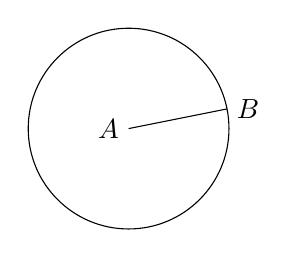
\begin{tikzpicture}
  \coordinate [label=left:$A$]  (A) at (0,0);
  \coordinate [label=right:$B$] (B) at (1.25,0.25);
  \draw (A) -- (B);

  \draw (A) let
              \p1 = ($ (B) - (A) $)
            in
              circle ({veclen(\x1,\y1)});
\end{tikzpicture}

    \end{column}
  \end{columns}

  \footnotesize
  \begin{enumerate}
    \item\pause een cirkel tekenen
      \mintinline{latex}|\draw (0,0) circle (1);|
    \item\pause we berekenen de co\"ordinaten voor $B-A$ (\texttt{let \ldots\ in} is met variabelen werken)
  \end{enumerate}
  \pause
  \begin{block}{Volgende stap}
    Nu nog de tweede cirkel.
  \end{block}
\end{frame}

\begin{frame}[fragile]
  \frametitle{Euclides: de cirkels rond $A$ en $B$ (2)}

  \begin{columns}
    \begin{column}{.67\textwidth}
      \inputminted[fontsize = \scriptsize]{latex}{tikz/triangle/2b.tikz}
    \end{column}
    \begin{column}{.33\textwidth}
      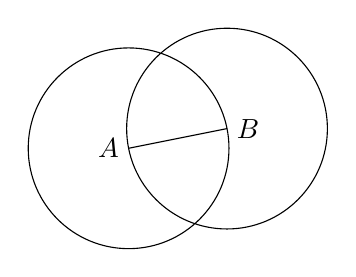
\begin{tikzpicture}
  \coordinate[label=left:$A$]  (A) at (0,0);
  \coordinate[label=right:$B$] (B) at (1.25,0.25);
  \draw (A) -- (B);

  \draw let \p1 = ($ (B) - (A) $),
            \n2 = {veclen(\x1,\y1)}
        in
          (A) circle (\n2)
          (B) circle (\n2);
\end{tikzpicture}

    \end{column}
  \end{columns}

  \footnotesize
  \begin{enumerate}
    \item\pause \mintinline{latex}|\p1| zijn co\"ordinaten, \mintinline{latex}|\n1| is een getal
    \item\pause \'e\'en \mintinline{latex}|\draw| kan meerdere zaken tekenen
  \end{enumerate}
  \pause
  \begin{block}{Volgende stap}
    We kunnen echter ook meteen cirkels door punten tekenen.
  \end{block}
\end{frame}

\begin{frame}[fragile]
  \frametitle{Euclides: de cirkels rond $A$ en $B$ (3)}

  \begin{columns}
    \begin{column}{.67\textwidth}
      \inputminted[fontsize = \scriptsize]{latex}{tikz/triangle/2c.tikz}
    \end{column}
    \begin{column}{.33\textwidth}
      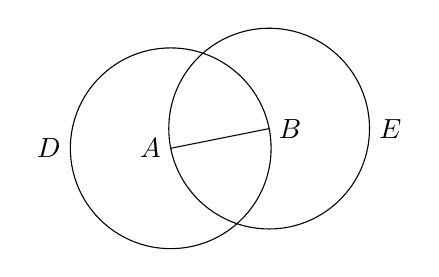
\begin{tikzpicture}
  \coordinate[label=left:$A$]  (A) at (0,0);
  \coordinate[label=right:$B$] (B) at (1.25,0.25);
  \draw (A) -- (B);

  \node[draw,circle through=(B),label=left:$D$]
    at (A) {};
  \node[draw,circle through=(A),label=right:$E$]
    at (B) {};
\end{tikzpicture}

    \end{column}
  \end{columns}

  \footnotesize
  \begin{enumerate}
    \item \mintinline{latex}|\node| is een combinatie van \mintinline{latex}|\coordinate| en \mintinline{latex}|\draw|
    \item de lege accolades zouden gebruikt kunnen worden voor tekst
  \end{enumerate}
  \pause
  \begin{block}{Volgende stap}
    Het snijpunt bepalen.
  \end{block}
\end{frame}

\begin{frame}
  \frametitle{Euclides: het snijpunt (1)}

  \begin{columns}
    \begin{column}{.67\textwidth}
      \inputminted[fontsize = \scriptsize]{latex}{tikz/triangle/3a.tikz}
    \end{column}
    \begin{column}{.33\textwidth}
      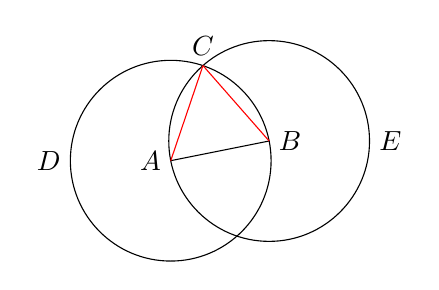
\begin{tikzpicture}
  \coordinate[label=left:$A$]  (A) at (0,0);
  \coordinate[label=right:$B$] (B) at (1.25,0.25);
  \draw (A) -- (B);

  \node (D) [name path=D,draw,circle through=(B),
             label=left:$D$]  at (A) {};
  \node (E) [name path=E,draw,circle through=(A),
             label=right:$E$] at (B) {};

  \path[name intersections={of=D and E}];

  \coordinate[label=above:$C$] (C) at (intersection-1);

  \draw[red] (A) -- (C);
  \draw[red] (B) -- (C);
\end{tikzpicture}

    \end{column}
  \end{columns}
\end{frame}

\begin{frame}[fragile]
  \frametitle{Euclides: het snijpunt (2)}

  \begin{enumerate} 
    \item we berekenen een \mintinline{latex}|\path| (= een reeks lijnsegmenten), dus in dit geval het (unieke) lijnstuk tussen de doorsnedes
    \item\pause we hebben de variabelen \texttt{intersection-1} en \texttt{intersection-2} die aangemaakt worden door de \texttt{intersections} library
    \item\pause we introduceren de naam \texttt{C} en tekenen twee lijnstukken
  \end{enumerate}
\end{frame}

\begin{frame}
  \frametitle{Euclides: de driehoek}

  \begin{columns}
    \begin{column}{.67\textwidth}
      \inputminted[fontsize = \scriptsize]{latex}{tikz/triangle/4a.tikz}
    \end{column}
    \begin{column}{.33\textwidth}
      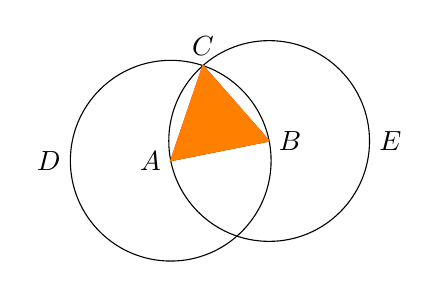
\begin{tikzpicture}
  \coordinate [label=left:$A$]  (A) at (0,0);
  \coordinate [label=right:$B$] (B) at (1.25,0.25);
  \draw (A) -- (B);

  \node (D) [name path=D,draw,circle through=(B),
             label=left:$D$]  at (A) {};
  \node (E) [name path=E,draw,circle through=(A),
             label=right:$E$] at (B) {};

  \path [name intersections={of=D and E}];

  \coordinate [label=above:$C$] (C) at (intersection-1);

  \draw [red] (A) -- (C);
  \draw [red] (B) -- (C);

  \draw [orange, fill] (A) -- (B) -- (C) -- cycle;
\end{tikzpicture}

    \end{column}
  \end{columns}
\end{frame}

\begin{frame}[fragile]
  \frametitle{Euclides: perfectioneren}

  \begin{enumerate}
    \item we gebruiken variabelen voor de kleuren:
      \begin{minted}{latex}
\colorlet{input}{blue!80!black}
\colorlet{triangle}{orange!80!white}
\colorlet{output}{red!70!black}
      \end{minted}
      (en passen de code aan)
    \item\pause we tekenen onze punten:
      \begin{minted}{latex}
\foreach \point in {A,B,C}
  \fill [black,opacity=.5] (\point) circle (2pt);
      \end{minted}
  \end{enumerate}
\end{frame}

\begin{frame}
  \frametitle{Euclides: het resultaat}

  \centering
  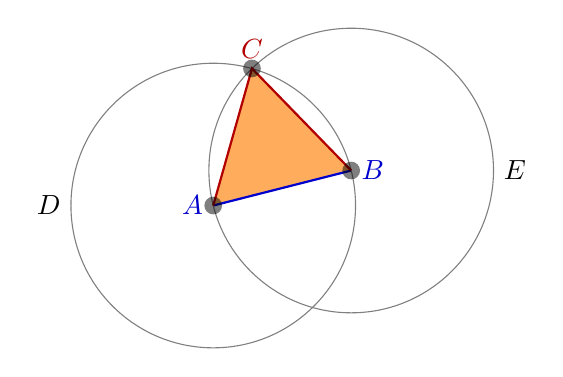
\begin{tikzpicture}[scale=1.6,thick,help lines/.style={thin,draw=black!50}]
  \def\A{\textcolor{input}{$A$}}
  \def\B{\textcolor{input}{$B$}}
  \def\C{\textcolor{output}{$C$}}
  \def\D{$D$}
  \def\E{$E$}

  \colorlet{input}{blue!80!black}
  \colorlet{triangle}{orange!80!white}
  \colorlet{output}{red!70!black}

  \coordinate [label=left:\A]  (A) at ($ (0,0) + .1*(rand,rand) $);
  \coordinate [label=right:\B] (B) at ($ (1.25,0.25) + .1*(rand,rand) $);

  \draw [input] (A) -- (B);

  \node [name path=D,help lines,draw,label=left:\D]
    (D) at (A) [circle through=(B)] {};
  \node [name path=E,help lines,draw,label=right:\E]
    (E) at (B) [circle through=(A)] {};

  \path [name intersections={of=D and E,by={[label=above:\C]C}}];

  \draw [output] (A) -- (C) -- (B);

  \foreach \point in {A,B,C}
    \fill [black,opacity=.5] (\point) circle (2pt);

  \begin{pgfonlayer}{background}
    \fill[triangle!80] (A) -- (C) -- (B) -- cycle;
  \end{pgfonlayer}
\end{tikzpicture}


\end{frame}

\begin{frame}
  \frametitle{Herhaling belangrijke zaken}

  \begin{enumerate}
    \item \mintinline{latex}|\draw| (eigenlijk \mintinline{latex}|\path[draw]|) om zaken te tekenen
    \item \mintinline{latex}|\coordinate| om co\"ordinaten op te slaan
    \item een lijn tekenen: \mintinline{latex}|\draw (0,0) -- (0,1);|
    \item een label toevoegen: \mintinline{latex}|\draw (0,0) -- (0,1) node {$f$};|
    \item opvullen: \mintinline{latex}|\draw[fill]|
    \item een cirkel: \mintinline{latex}|\draw (0,0) circle (2cm);|
  \end{enumerate}
\end{frame}

\begin{frame}
  \frametitle{Oefening}

  \centering
  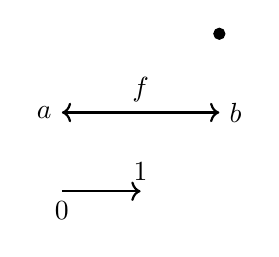
\begin{tikzpicture}
    \draw[thick, ->] (0,0) node [below] {$0$} -- (1,0) node [above] {$1$};
    \draw[thick, <->] (0,1) node [left] {$a$} to node[above]{$f$} (2,1) node [right] {$b$};
    \draw[fill] (2,2) circle (2pt);
  \end{tikzpicture}
\end{frame}

\begin{frame}[fragile]
  \frametitle{Oplossing}

  \begin{minted}{latex}
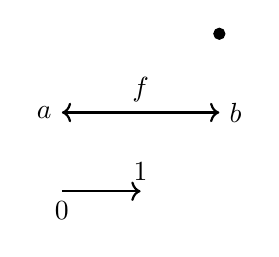
\begin{tikzpicture}
  \draw[thick, ->]
    (0,0) node[below] {$0$}
    --
    (1,0) node[above] {$1$};
  \draw[thick, <->]
    (0,1) node[left] {$a$}
    to node[above]{$f$}
    (2,1) node[right] {$b$};
  \draw[fill] (2,2) circle (2pt);
\end{tikzpicture}
  \end{minted}
\end{frame}


\begin{frame}
  \frametitle{Functies plotten}
\end{frame}

\begin{frame}
  \frametitle{Datasets plotten}
\end{frame}

\begin{frame}
  \frametitle{Contour plots}

  \centering
  \begin{tikzpicture}[scale = .5]
  \begin{axis}[
    colormap name=whitered,
    3d box,
    width=15cm,
    view={25}{25},
    enlargelimits=false,
    grid=major,
    domain=-0.5:4.7,
    y domain=-2:2,
    samples=21,
    xlabel=$x$,
    ylabel=$\dot{x}$,
    zlabel={$\text{E}_{\text{m}}$},
    colorbar,
    colorbar style={
        at={(1,0)},
        anchor=south west,
        height=0.1*\pgfkeysvalueof{/pgfplots/parent axis height},
        title={$\text{E}_{\text{m}}(x,\dot{x})$}
        },
    colormap={whitered}{color(0cm)=(white); color(1cm)=(orange!75!red)}
    ]
    \addplot3 [y domain = 0:2, surf]
      {-0.7+4*exp(-0.5*(x+3))*(3*cos(4*x*180/pi)+2.5*cos(2*x*180/pi))
       + 0.5*y*y*4};

    \addplot3 [y domain = 0:2, contour gnuplot = {number=14, labels={false},
      draw color = ugentblue}, samples = 21, ]
      {-0.7+4*exp(-0.5*(x+3))*(3*cos(4*x*180/pi)+2.5*cos(2*x*180/pi))
       + 0.5*y*y*4};

    \addplot3 [domain = -0.5:4.7, samples = 31, samples y = 0, thick, smooth]
        (x,-2,{-0.6+4*exp(-0.5*(x+3))*(3*cos(4*x*180/pi)+2.5*cos(2*x*180/pi))});
    \addplot3 [contour gnuplot = {number=14, labels={false}, draw color=ugentblue},
        samples=21,z filter/.code={\def\pgfmathresult{20}}]
        {-0.7+4*exp(-0.5*(x+3))*(3*cos(4*x*180/pi)+2.5*cos(2*x*180/pi))
         + 0.5*y*y*4};
    \addplot3 [y domain=-2:0,surf]
        {-0.7+4*exp(-0.5*(x+3))*(3*cos(4*x*180/pi)+2.5*cos(2*x*180/pi))
         + 0.5*y*y*4};
    \addplot3 [domain = 0:.25, contour gnuplot = {number=14,labels={false},
        draw color=ugentblue}, samples=21]
        {-0.7+4*exp(-0.5*(x+3))*(3*cos(4*x*180/pi)+2.5*cos(2*x*180/pi))
         + 0.5*y*y*4};
  \end{axis}
\end{tikzpicture}


  \small\url{http://pgfplots.net/tikz/examples/contour-surface/}
\end{frame}

\begin{frame}
  \frametitle{Weierstrassfunctie}

  \centering
  \begin{luacode}
  function weierstrass(x0, x1, n, a, b, epsilon)
    local dx = (x1-x0)/n 
    local x = x0
    local out=assert(io.open("tmp.data","w"))
    local y,k,dy
    while (x <= x1) do
      y = 0
      k = 0
      repeat
        dy = math.pow(a,k) * math.cos(math.pow(b,k)*math.pi*x)
        y = y + dy
        k = k + 1
      until (math.abs(dy) < epsilon)
      out:write(x, " ", y, "\string\n") 
      x = x + dx
    end
    out:close()
  end
\end{luacode}

\begin{tikzpicture}[every pin/.style={fill=white},pin distance=1.2cm]
  \directlua{weierstrass(-2,2,5000,0.3,5,1.e-12)}%
  \begin{axis}[axis lines=middle,domain=-2:2]
    \addplot [thin, line join=round] table {tmp.data};
    \coordinate (p1) at (axis cs:1,-1.38);
    \coordinate (p2) at (axis cs:1.8,0.6);
    \coordinate (legend) at (axis cs:0,2);
  \end{axis}
  \directlua{weierstrass(0.95,1.05,5000,0.3,5,1.e-12)}%
  \node[pin=3:{%
    \begin{tikzpicture}[baseline,trim axis left,trim axis right]
      \begin{axis}[tiny,axis lines=box,domain=0.95:1.05,scale=0.5]
        \addplot [thin, line join=round] table {tmp.data};
      \end{axis}
    \end{tikzpicture}%
  }] at (p1) {};
  \directlua{weierstrass(1.7,1.9,5000,0.3,5,1.e-12)}%
  \node[pin=3:{%
    \begin{tikzpicture}[baseline,trim axis left,trim axis right]
      \begin{axis}[tiny,axis lines=box,domain=1.7:1.9]
        \addplot [thin, line join=round] table {tmp.data};
      \end{axis}
    \end{tikzpicture}%
  }] at (p2) {};
  \node at (legend)
    {$\displaystyle f(x) = \sum_{n=0}^\infty a^n \cos(b^n \pi x)$};
\end{tikzpicture}


  \small\url{http:/pgfplots.net/tikz/examples/weierstrass-function/}
\end{frame}



\section{Uitbeidingen op TikZ}

\begin{frame}
  \frametitle{Libraries}

  Zie \S IV in versie 2.10, of \S V in versie 3.0 voor de \emph{libraries} (= intern).

  \pause
  Te gebruiken via:
  
  \mintinline{latex}|\usetikzlibrary{lindenmayersystems}|

  \begin{alertblock}{Vraag}
    Wat doet deze library?
  \end{alertblock}
\end{frame}

\begin{frame}
  \frametitle{Lindenmayersystemen}

  \begin{columns}
    \begin{column}{.6\textwidth}
      \inputminted[fontsize = \scriptsize]{latex}{tikz/l-system.tikz}
    \end{column}
    \begin{column}{.4\textwidth}
      \begin{tikzpicture}
\draw[green!50!black, rotate=90]
  [l-system={rule set={F -> FF-[-F+F]+[+F-F]},
    axiom=F, order=4, step=2pt,
    randomize step percent=25, angle=30,
    randomize angle percent=5}]
  lindenmayer system;
\end{tikzpicture}

    \end{column}
  \end{columns}
\end{frame}

\begin{frame}
  \frametitle{Packages}

  Zie \url{http://ctan.org/search?phrase=tikz} voor \emph{packages} (= extern): 90+ resultaten

  \mintinline{latex}|\usepackage{...}|

  \pause
  \begin{enumerate}
    \item \texttt{tikz-qtree}
    \item \texttt{tqft}
    \item \texttt{tikz-cd}
    \item \ldots
  \end{enumerate}
\end{frame}

\begin{frame}
  \frametitle{\texttt{tikz-qtree}}
  
  Automatisch bomen tekenen:
  \begin{columns}
    \begin{column}{.6\textwidth}
      \inputminted[fontsize = \scriptsize]{latex}{tikz/tikz-qtree.tikz}
    \end{column}
    \begin{column}{.4\textwidth}
      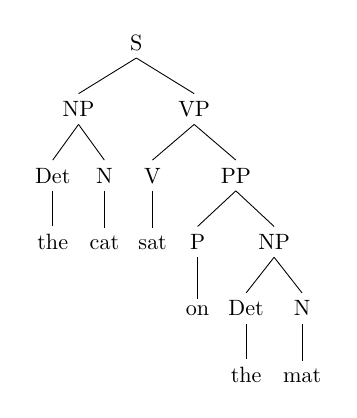
\begin{tikzpicture}[scale = .8]
  \Tree [.S [.NP [.Det the ] [.N cat ] ]
            [.VP [.V sat ]
                 [.PP [.P on ]
                      [.NP [.Det the ]
                      [.N mat ] ] ] ] ]
\end{tikzpicture}

    \end{column}
  \end{columns}
\end{frame}

\begin{frame}
  \frametitle{\texttt{tqft}}
  
  Om diagrammen in topologische quantumveldentheorie te tekenen:
  \begin{columns}
    \begin{column}{.6\textwidth}
      \inputminted[fontsize = \scriptsize]{latex}{tikz/tqft.tikz}
    \end{column}
    \begin{column}{.4\textwidth}
      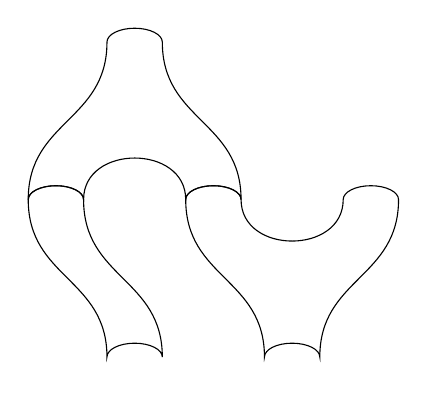
\begin{tikzpicture}[scale = .8]
  \node[draw, tqft/pair of pants]
    (a) {};
  \node[draw, tqft/cylinder to next,
        anchor = incoming boundary 1]
    (c) at (a.outgoing boundary 1) {};
  \node[draw, tqft/reverse pair of pants,
        anchor = incoming boundary 1]
    at (a.outgoing boundary 2) (b) {};
\end{tikzpicture}

    \end{column}
  \end{columns}
\end{frame}

\begin{frame}
  \frametitle{\texttt{rubikcube}}

  Om Rubik's cubes te tekenen:
  \begin{columns}
    \begin{column}{.6\textwidth}
      \inputminted[fontsize = \scriptsize]{latex}{tikz/rubikcube.tikz}
    \end{column}
    \begin{column}{.4\textwidth}
      
\begin{tikzpicture}[scale=.4]
  \DrawRubikLayerFace{G}{Y}{R}
                     {Y}{Y}{Y}
                     {B}{Y}{Y}
  \DrawRubikLayerSideT {Y}{B}{B}
  \DrawRubikLayerSideLR{R}   {Y}
                       {R}   {O}
                       {Y}   {O}
  \DrawRubikLayerSideB {O}{G}{G}
  \draw[->,ultra thick,color=green]
    (0.5,5) -- (0.5, 4);
\end{tikzpicture}

\begin{tikzpicture}[scale=.4]
  \RubikCubeSolved
  \DrawRubikCubeFlat
\end{tikzpicture}

    \end{column}
  \end{columns}
\end{frame}

\subsection{Commutatieve diagrammen}

\begin{frame}[fragile]
  \frametitle{Commutatieve diagrammen}

  \small
  We gebruiken \mintinline{latex}|\usepackage{tikz-cd}|.
  \begin{columns}
    \begin{column}{.67\textwidth}
      \inputminted[fontsize = \scriptsize]{latex}{tikz/diagrams/1.tikz}
    \end{column}
    \begin{column}{.33\textwidth}
      \begin{equation*}
  \begin{tikzcd}
    A \arrow{rd} \arrow{r}{\phi} & B \\
                                 & C
  \end{tikzcd}
\end{equation*}

    \end{column}
  \end{columns}
  \small
  \begin{enumerate}
    \item\pause de \emph{eerste parameter} van \mintinline{latex}|\arrow| is altijd de richting: een combinatie van \texttt{u}, \texttt{d}, \texttt{r}, \texttt{l}, de \emph{tweede} een (optioneel) label
    \item\pause vertices zoals we tabellen schrijven 
  \end{enumerate}
  \begin{alertblock}{Opgepast}
    \dbend\quad Pijlen kunnen enkel naar bestaande vertices.
  \end{alertblock}
\end{frame}

\begin{frame}
  \frametitle{Oefening}

  \footnotesize
  \begin{equation*}
  \begin{tikzcd}
    A  \arrow{r}{f} \arrow{d}{l} & B \arrow{r}{g} \arrow{d}{m} & C \arrow{r}{h} \arrow{d}{n} & D \arrow{r}{j} \arrow{d}{p} & E \arrow{d}{q} \\
    A' \arrow[swap]{r}{r}        & B' \arrow[swap]{r}{s}       & C' \arrow[swap]{r}{t}       & D' \arrow[swap]{r}{u}       & E' \\
  \end{tikzcd}
\end{equation*}

  \begin{equation*}
  \begin{tikzcd}
    T
    \arrow{drr}{x}
    \arrow[swap]{ddr}{y}
    \arrow[dotted]{dr}[description]{\exists} & & \\
      & X \times_Z Y \arrow[swap]{r}{p} \arrow{d}{q}
        & X \arrow{d}{f} \\
      & Y \arrow[swap]{r}{g} &Z
  \end{tikzcd}
\end{equation*}

\end{frame}


\end{document}
